\chapter{Two-view geometry}
\label{ch:twoview}

Two images of a rigid scene, taken from different places, are not
independent: the second camera must see each point somewhere along a
line determined by where the first camera saw it. This chapter derives
that constraint, shows how the relative motion of the cameras can be
read from it, recovers the 3D points by triangulation, and studies when
all of this breaks down. Two of those failure modes, a planar scene and
a camera that turns without moving, describe a mower on a lawn rather
well, so the last section is the most important one for us.

Throughout, image points are in normalised coordinates
$\vect{x}=\pi(\vect{q})$ (pixels mapped through $K^{-1}$ and
undistorted, Chapter~\ref{ch:cameras}), with $\tilde{\vect{x}}=
(\vect{x},1)$. The relative pose $(R,\vect{t})$ maps coordinates in
camera~1 to coordinates in camera~2: $\vect{q}_2=R\vect{q}_1+\vect{t}$.
In terms of poses, $(R,\vect{t})=T_{c_2c_1}=T_{wc_2}^{-1}T_{wc_1}$.

\section{The epipolar constraint}

\begin{figure}[ht]
\centering
\begin{tikzpicture}[scale=1.1,>=Stealth]
\coordinate (C1) at (0,0);
\coordinate (C2) at (5,0.3);
\coordinate (X) at (2.6,3.4);
\draw[fill=defblue!8,draw=defblue] (0.3,0.9) -- (1.6,1.4) -- (1.6,2.6)
  -- (0.3,2.1) -- cycle;
\draw[fill=defblue!8,draw=defblue] (3.6,1.4) -- (4.8,0.9) -- (4.8,2.2)
  -- (3.6,2.7) -- cycle;
\fill (C1) circle (1.5pt) node[below left] {$\vect{c}_1$};
\fill (C2) circle (1.5pt) node[below right] {$\vect{c}_2$};
\fill (X) circle (1.8pt) node[above] {$\p$};
\draw[thick] (C1) -- (X) -- (C2);
\draw[dashed] (C1) -- (C2) node[midway,below] {baseline $\vect{t}$};
\coordinate (x1) at ($(C1)!0.43!(X)$);
\coordinate (x2) at ($(C2)!0.43!(X)$);
\fill[thmred] (x1) circle (1.6pt) node[left] {$\vect{x}_1$};
\fill[thmred] (x2) circle (1.6pt) node[right] {$\vect{x}_2$};
\coordinate (e1) at ($(C1)!0.27!(C2)$);
\coordinate (e2) at ($(C2)!0.24!(C1)$);
\fill[wordsgreen] (e2) circle (1.6pt) node[below] {$\vect{e}_2$};
\fill[wordsgreen] (e1) circle (1.6pt) node[below] {$\vect{e}_1$};
\draw[wordsgreen,thick] (e2) -- ($(e2)!1.55!(x2)$)
  node[right,font=\small] {epipolar line $E\tilde{\vect{x}}_1$};
\fill[lawngreen!12,opacity=0.5] (C1) -- (X) -- (C2) -- cycle;
\end{tikzpicture}
\caption{Epipolar geometry. The two optical centres and the point $\p$
span the epipolar plane. Whatever the depth of $\p$ along the ray of
$\vect{x}_1$, its image in camera~2 lies on the intersection of that
plane with the image: the epipolar line. All epipolar lines pass
through the epipole $\vect{e}_2$, the image of $\vect{c}_1$.}
\label{fig:epipolar}
\end{figure}

\begin{proposition}{The epipolar constraint}{epipolar}
If $\vect{q}_1$ and $\vect{q}_2=R\vect{q}_1+\vect{t}$ are the coordinates
of one point in the two camera frames, with images $\vect{x}_1,
\vect{x}_2$, then
\begin{equation}\label{eq:epipolar}
\tilde{\vect{x}}_2\T E\,\tilde{\vect{x}}_1=0,\qquad E=\hatop{\vect{t}}R .
\end{equation}
In pixels, $\tilde{\vect{u}}_2\T F\tilde{\vect{u}}_1=0$ with the
\emph{fundamental matrix} $F=K_2^{-\mathsf T}EK_1^{-1}$.
\end{proposition}

\begin{proof}
$\vect{q}_2$, $\vect{t}$ and $R\vect{q}_1$ are linearly dependent, since
$\vect{q}_2-R\vect{q}_1-\vect{t}=\vect0$; hence their triple product
vanishes: $\vect{q}_2\T(\vect{t}\times R\vect{q}_1)=\vect{q}_2\T
\hatop{\vect{t}}R\vect{q}_1=0$. Divide by the depths $Z_1Z_2>0$, using
$\vect{q}_i=Z_i\tilde{\vect{x}}_i$. For pixels, substitute
$\tilde{\vect{x}}_i=K_i^{-1}\tilde{\vect{u}}_i$.
\end{proof}

\begin{definition}{Epipoles and epipolar lines}{epipoles}
The \emph{epipole} $\vect{e}_2$ is the image in camera~2 of the centre of
camera~1, $\vect{e}_2\sim\vect{t}$; symmetrically $\vect{e}_1\sim
-R\T\vect{t}$. The \emph{epipolar line} of $\vect{x}_1$ in image~2 is the
set of $\vect{x}$ with $\tilde{\vect{x}}\T\vect{l}_2=0$, $\vect{l}_2=E
\tilde{\vect{x}}_1$. One has $\vect{e}_2\T E=\vect0$ and $E\vect{e}_1=
\vect0$, so every epipolar line of image~2 passes through $\vect{e}_2$
(Exercise~\ref{ex:6epi}).
\end{definition}

\begin{inwords}
Matching becomes a one-dimensional search: given $\vect{x}_1$, look for
its partner along a line, not over the whole image. And every
correspondence gives one scalar equation in the unknown motion. Note
what the constraint does \emph{not} see: multiplying $\vect{t}$ by any
$\lambda>0$ leaves \eqref{eq:epipolar} unchanged. Two images determine
the direction of translation, never its length --- the monocular scale
gauge of Chapter~\ref{ch:slam}, once more.
\end{inwords}

\section{The essential matrix}

\begin{theorem}{Characterisation of essential matrices}{essential}
A nonzero $3\times3$ matrix is of the form $\hatop{\vect{t}}R$ with
$R\in\SO3$, $\vect{t}\neq\vect0$, if and only if its singular values are
$(\sigma,\sigma,0)$ with $\sigma>0$.
\end{theorem}

\begin{proof}
($\Rightarrow$) $EE\T=\hatop{\vect{t}}RR\T(\hatop{\vect{t}})\T=
-(\hatop{\vect{t}})^2=\norm{\vect{t}}^2I-\vect{t}\vect{t}\T$ by
\cref{lem:hatid}(ii). Its eigenvalues are $\norm{\vect{t}}^2$ (twice, on
$\vect{t}^\perp$) and $0$ (on $\vect{t}$), so the singular values of $E$
are $\norm{\vect{t}},\norm{\vect{t}},0$.

($\Leftarrow$) Let $E=U\diag(\sigma,\sigma,0)V\T$. Since the third
singular value is zero, we may change the sign of the third column of
$U$ or of $V$ without changing $E$, and so assume $U,V\in\SO3$. With
\[
W=\begin{pmatrix}0&-1&0\\1&0&0\\0&0&1\end{pmatrix},\qquad
Z=\begin{pmatrix}0&1&0\\-1&0&0\\0&0&0\end{pmatrix},
\]
one checks $ZW=\diag(1,1,0)$, so $E=\sigma\,(UZU\T)(UWV\T)$. Here
$UWV\T\in\SO3$, and $UZU\T$ is skew-symmetric since $Z$ is; precisely,
$Z=-\hatop{\vect{e}_3}$ and \cref{lem:hatid}(v) give $\sigma UZU\T=
\hatop{(-\sigma\vect{u}_3)}$, where $\vect{u}_3$ is the third column of
$U$. Hence $E=\hatop{\vect{t}}R$ with $\vect{t}=-\sigma\vect{u}_3$ and
$R=UWV\T$.
\end{proof}

An essential matrix therefore has five degrees of freedom: three for the
rotation and two for the direction of translation, its scale being
irrelevant.

\begin{proposition}{The four decompositions}{decompose}
Let $E=U\diag(1,1,0)V\T$ with $U,V\in\SO3$. The pairs $(R,\vect{t})$
with $\norm{\vect{t}}=1$ and $\hatop{\vect{t}}R=\pm E$ are exactly
\[
(UWV\T,\ \pm\vect{u}_3),\qquad(UW\T V\T,\ \pm\vect{u}_3).
\]
For a correspondence in general position, exactly one of the four
places the triangulated point in front of both cameras.
\end{proposition}

\begin{proof}
$E\T\vect{t}=R\T(\hatop{\vect{t}})\T\vect{t}=-R\T(\vect{t}\times\vect{t})
=\vect0$, so $\vect{t}$ spans the left null space of $E$, which is
spanned by $\vect{u}_3$: $\vect{t}=\pm\vect{u}_3$. Take $\vect{t}=
-\vect{u}_3$, so $\hatop{\vect{t}}=UZU\T$ (proof of \cref{thm:essential}),
and write the unknown rotation as $R=UXV\T$ with $X\in\SO3$. The
equation $\hatop{\vect{t}}R=E$ becomes $ZX=ZW$, i.e.\ $Z(X-W)=0$: every
column of $X-W$ lies in the null space of $Z$, which is spanned by
$\vect{e}_3$. So $X$ and $W$ share their first two rows, $(0,-1,0)$ and
$(1,0,0)$, and the third row of $X$, a unit vector orthogonal to both,
is $(0,0,\pm1)$; $\det X=1$ forces $X=W$. The equation
$\hatop{\vect{t}}R=-E$ gives in the same way $Z(X+W)=0$ and $X=W\T$.
Changing the sign of $\vect{t}$ exchanges $E$ and $-E$, which yields the
four pairs. The cheirality statement is the geometric fact, shown in
\cref{fig:fourfold}, that the four configurations differ by swapping
the cameras' positions along the baseline and by a half-turn of camera~2
about it, and only one of them puts a given point in front of both
cameras (Hartley and Zisserman, Result 9.19).
\end{proof}

\begin{figure}[ht]
\centering
\begin{tikzpicture}[scale=0.75,>=Stealth,
  cam/.style={fill=defblue,draw=defblue},
  lab/.style={font=\small,align=center}]
\foreach \dx/\bx/\bs/\px/\py/\ok/\name/\txt in {
  0/2/1/1/1.6/1/(a)/in front of both,
  5.5/-2/1/-1/-1.6/0/(b)/behind both,
  11/2/-1/1/1.6/0/(c)/behind camera 2,
  16.5/-2/-1/-1/-1.6/0/(d)/behind camera 1}{
  \begin{scope}[xshift=\dx cm]
  \draw[gray!60] (-2.4,0) -- (2.4,0);
  \draw[gray] (0,0) -- (\px,\py) -- (\bx,0);
  \draw[thick,->] (0,0) -- (0,0.9);
  \draw[thick,->] (\bx,0) -- (\bx,0.9*\bs);
  \fill[cam] (0,0) circle (2.5pt) node[below left,font=\scriptsize] {1};
  \fill[cam] (\bx,0) circle (2.5pt) node[below right,font=\scriptsize]
    {2};
  \ifnum\ok=1 \fill[wordsgreen] (\px,\py) circle (3pt);
  \else \fill[thmred] (\px,\py) circle (3pt); \fi
  \node[lab] at (0,-2.4) {\name\ \txt};
  \end{scope}}
\end{tikzpicture}
\caption{The fourfold ambiguity, schematically, after Hartley and
Zisserman (dots: cameras, arrows: optical axes, disc: the triangulated
point). From (a), reversing the baseline gives (b); turning camera~2 by
a half-turn about the baseline gives (c), the ``twisted pair''; doing
both gives (d). Only (a) has the point in front of both cameras.}
\label{fig:fourfold}
\end{figure}

\section{Estimating the essential matrix}

\paragraph{The eight-point algorithm.} Equation \eqref{eq:epipolar} is
linear in the nine entries of $E$: $\tilde{\vect{x}}_2\T E\tilde{
\vect{x}}_1=(\tilde{\vect{x}}_2\otimes\tilde{\vect{x}}_1)\T\vect{e}$
with $\vect{e}$ the rows of $E$ stacked. Eight correspondences or more
give a homogeneous system $A\vect{e}=\vect0$, solved by the smallest
right singular vector of $A$ exactly as the DLT of \cref{prop:dlt},
after Hartley normalisation. The result is not an essential matrix in
general; it is replaced by the closest one in Frobenius norm, which, if
$\hat E=U\diag(s_1,s_2,s_3)V\T$, is $U\diag(\bar s,\bar s,0)V\T$ with
$\bar s=(s_1+s_2)/2$ (a consequence of von Neumann's trace inequality).
Since $E$ is defined up to scale we use $\diag(1,1,0)$.

\begin{proposition}{The cubic constraints}{demazure}
Every essential matrix satisfies $\det E=0$ and the nine cubic equations
\[
2\,EE\T E-\tr(EE\T)\,E=0 .
\]
\end{proposition}

\begin{proof}
With $E=U\diag(\sigma,\sigma,0)V\T$, $\det E=0$, $EE\T E=\sigma^3U\diag(
1,1,0)V\T=\sigma^2E$ and $\tr(EE\T)=2\sigma^2$, so the left-hand side is
$2\sigma^2E-2\sigma^2E=0$.
\end{proof}

\paragraph{The five-point algorithm.} Five degrees of freedom suggest
that five correspondences should suffice, and they do. Five equations
$A\vect{e}=\vect0$ leave a four-dimensional null space,
$E=\alpha_1E_1+\alpha_2E_2+\alpha_3E_3+E_4$; substituting into the
constraints of \cref{prop:demazure} gives ten cubic equations in
$(\alpha_1,\alpha_2,\alpha_3)$, which Nist\'er reduces to a polynomial
of degree ten. Up to ten real solutions are returned and RANSAC keeps
the one with the largest consensus. We do not rederive the solver; the
code calls OpenCV's implementation (\code{cv2.findEssentialMat}). What
matters is the sample size: by the table of Chapter~\ref{ch:features},
five instead of eight is the difference between a feasible and an
infeasible RANSAC when many matches are wrong, and the five-point
algorithm, unlike the eight-point one, uses the constraints of
\cref{prop:demazure} rather than ignoring them --- which is why planar
scenes do not wreck it the way they wreck the eight-point algorithm,
although \cref{sec:degenerate} shows it is not immune either.

\paragraph{The error to minimise.} The algebraic residual
$\tilde{\vect{x}}_2\T E\tilde{\vect{x}}_1$ has no geometric meaning. A
better residual for RANSAC and for refinement is:

\begin{proposition}{Sampson distance}{sampson}
Let $\epsilon=\tilde{\vect{x}}_2\T E\tilde{\vect{x}}_1$ and $\vect{j}\in
\R^4$ its gradient with respect to $(\vect{x}_1,\vect{x}_2)$,
$\vect{j}=\bigl((E\T\tilde{\vect{x}}_2)_{1:2},\ (E\tilde{\vect{x}}_1)_{
1:2}\bigr)$. To first order, the smallest perturbation of the
correspondence that satisfies the epipolar constraint has norm
\[
d_S=\frac{|\epsilon|}{\norm{\vect{j}}}=\frac{|\tilde{\vect{x}}_2\T
E\tilde{\vect{x}}_1|}{\sqrt{(E\tilde{\vect{x}}_1)_1^2+(E\tilde{
\vect{x}}_1)_2^2+(E\T\tilde{\vect{x}}_2)_1^2+(E\T\tilde{\vect{x}}_2)_2^2
}} .
\]
\end{proposition}

\begin{proof}
Linearise: a perturbation $\vect\delta\in\R^4$ changes $\epsilon$ into
$\epsilon+\vect{j}\T\vect\delta$. The minimum-norm $\vect\delta$ with
$\epsilon+\vect{j}\T\vect\delta=0$ is the projection
$\vect\delta=-\epsilon\vect{j}/\norm{\vect{j}}^2$, of norm $|\epsilon|/
\norm{\vect{j}}$.
\end{proof}

\section{Triangulation}

Given $(R,\vect{t})$, a correspondence defines two rays; with noise they
do not meet. The \emph{linear} (DLT) triangulation stacks the
constraints $\tilde{\vect{x}}_i\times P_i\tilde{\p}=\vect0$ with
$P_1=[I\ \vect0]$, $P_2=[R\ \vect{t}]$, keeps two independent rows per
view and takes the smallest singular vector of the resulting $4\times4$
system. It is the initial value; the optimal estimate minimises the
reprojection error in both images with the methods of
Chapter~\ref{ch:nls}, which is what bundle adjustment (Chapter~8) does
for all points at once.

\begin{proposition}{Depth accuracy and parallax}{parallax}
Let a point at depth $Z$ be seen from two centres a distance $b$ apart,
with pixel noise $\sigma$ in each image and focal length $f$.
\begin{enumerate}[label=(\roman*),nosep]
\item If the baseline is perpendicular to the line of sight, the
  parallax angle is $\theta\approx b/Z$ and, to first order,
  \[
  \frac{\sigma_Z}{Z}\approx\frac{\sqrt2\,\sigma}{f\,\theta} .
  \]
\item If the camera moves by $b$ along a direction making the angle
  $\alpha$ with the line of sight of a point at distance $\rho$, the
  parallax is $\theta\approx(b/\rho)\sin\alpha$.
\end{enumerate}
\end{proposition}

\begin{proof}
(i) This is the stereo configuration of \cref{prop:disparity}, with a
disparity that combines two independent pixel errors, hence
$\sigma_\delta=\sqrt2\sigma$: $\sigma_Z=Z^2\sqrt2\sigma/(fb)=Z\sqrt2
\sigma/(f\theta)$. (ii) In the triangle formed by the two centres and the
point, the angle at the point is $\theta$ and the side opposite to it is
$b$; by the law of sines, $\sin\theta=b\sin\alpha'/\rho'$ with
$\alpha'$, $\rho'$ the angle and distance seen from the second centre,
which equal $\alpha$, $\rho$ up to $O(b/\rho)$.
\end{proof}

\begin{inwords}
Depth error is inversely proportional to the angle between the two rays
(\cref{fig:triangulation}, left). And when the camera moves forward ---
as a mower does nearly all the time --- the parallax of a point is
proportional to its angular distance from the direction of motion
(the epipole): straight ahead there is none at all
(\cref{fig:triangulation}, right). Points near the centre of a
forward-looking image cannot be triangulated from forward motion, however
far the mower drives. Systems therefore create a new keyframe only when
enough points have reached a minimum parallax, typically one or two
degrees.
\end{inwords}

\begin{figure}[ht]
\centering
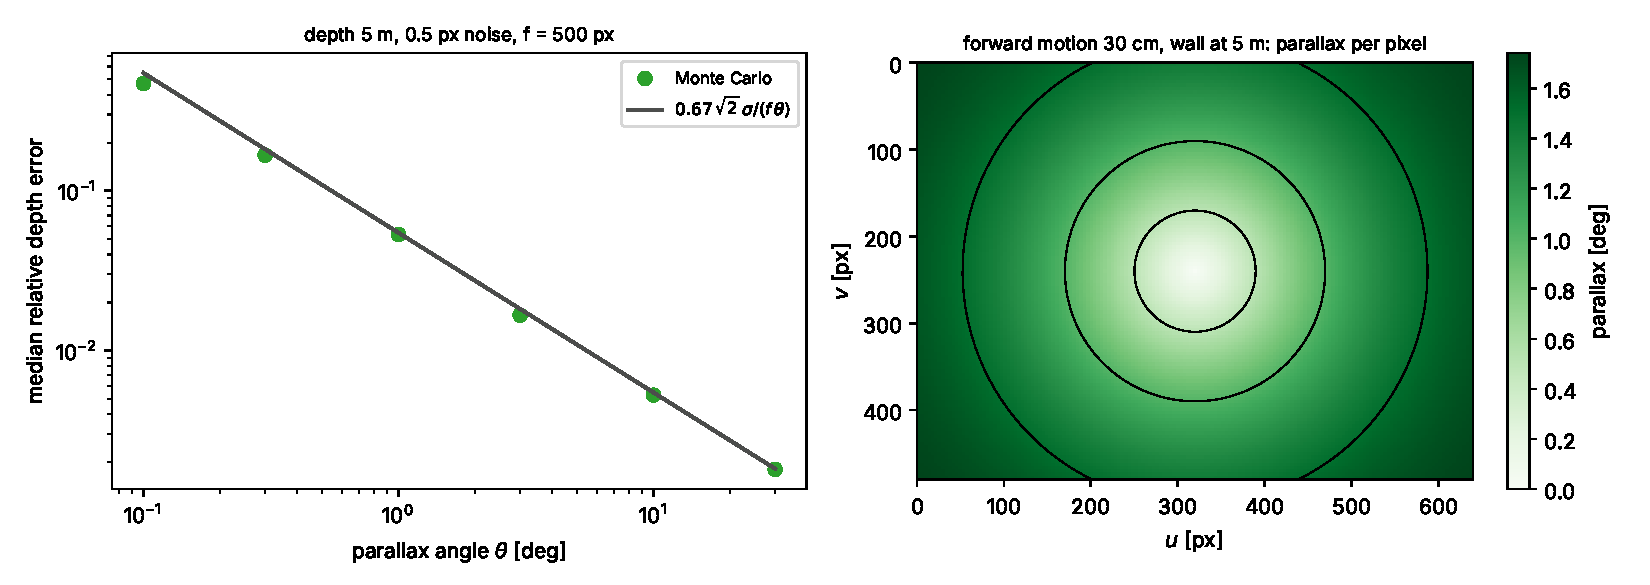
\includegraphics[width=\linewidth]{figures/ch06_triangulation.pdf}
\caption{Left: median relative depth error of DLT triangulation versus
parallax angle; dots: Monte Carlo, line: \cref{prop:parallax}(i) with
$0.67$, the median of $|\Normal(0,1)|$. Right: parallax of each pixel
after a 30\,cm forward motion, for a wall 5\,m ahead; contours at 0.5,
1 and 1.5 degrees.}
\label{fig:triangulation}
\end{figure}

\section{Degenerate configurations}
\label{sec:degenerate}

\subsection{A planar scene}

\begin{proposition}{Planar scenes}{planar}
Suppose all points lie on a plane $\vect{n}\T\vect{q}_1=d$ ($d>0$) of
camera~1. Then
\begin{enumerate}[label=(\roman*),nosep]
\item every correspondence satisfies $\tilde{\vect{x}}_2\sim H\tilde{
  \vect{x}}_1$ with $H=R+\vect{t}\vect{n}\T/d$;
\item for every $\vect{a}\in\R^3$, the matrix $\hatop{\vect{a}}H$
  satisfies \eqref{eq:epipolar} for all the correspondences, so the
  eight-point system has a null space of dimension at least three and
  determines nothing.
\end{enumerate}
\end{proposition}

\begin{proof}
(i) For a point of the plane, $\vect{n}\T\vect{q}_1/d=1$, so
$\vect{q}_2=R\vect{q}_1+\vect{t}=(R+\vect{t}\vect{n}\T/d)\vect{q}_1$;
divide by the depths. (ii) $\tilde{\vect{x}}_2\T\hatop{\vect{a}}H
\tilde{\vect{x}}_1=\lambda\,\tilde{\vect{x}}_2\T(\vect{a}\times
\tilde{\vect{x}}_2)=0$ with $\lambda\neq0$. The map
$\vect{a}\mapsto\hatop{\vect{a}}H$ is linear and injective when $H$ is
invertible, so its image is a three-dimensional space of solutions of
the eight-point system.
\end{proof}

Calibration helps, but not enough. The true $E$ is of the form
$\hatop{\vect{a}}H$ (with $\vect{a}=\vect{t}$: $\hatop{\vect{t}}H=
\hatop{\vect{t}}R$ since $\hatop{\vect{t}}\vect{t}=\vect0$), and among
this three-parameter family there are in general \emph{two} essential
matrices, both compatible with every correspondence and both placing
every point in front of both cameras (Longuet-Higgins, 1986). The
five-point algorithm returns one of them. On our simulated lawns it
returned the wrong ``twin'' in 20 to 33\,\% of the trials, with a
rotation error of about $20^\circ$, while never failing once the scene
had 10\,cm of relief (\cref{fig:degeneracy}, left).

The remedy is to use the model the data actually obey. A homography is
estimated from four points with the DLT and RANSAC of
Chapter~\ref{ch:features}, and decomposed into $(R,\vect{t}/d,\vect{n})$
(Faugeras and Lustman; Malis and Vargas): there are up to four
solutions, two of which pass the cheirality test. For a mower the tie is
broken by prior knowledge: the camera's height and tilt are known, so the
normal of the ground is known approximately, and the solution whose
$\vect{n}$ is closest to it is the right one. Which model to use is
decided by testing whether the homography explains (nearly) all
matches at the noise level; ORB-SLAM's initialisation does a scored
version of this test.

\begin{figure}[ht]
\centering
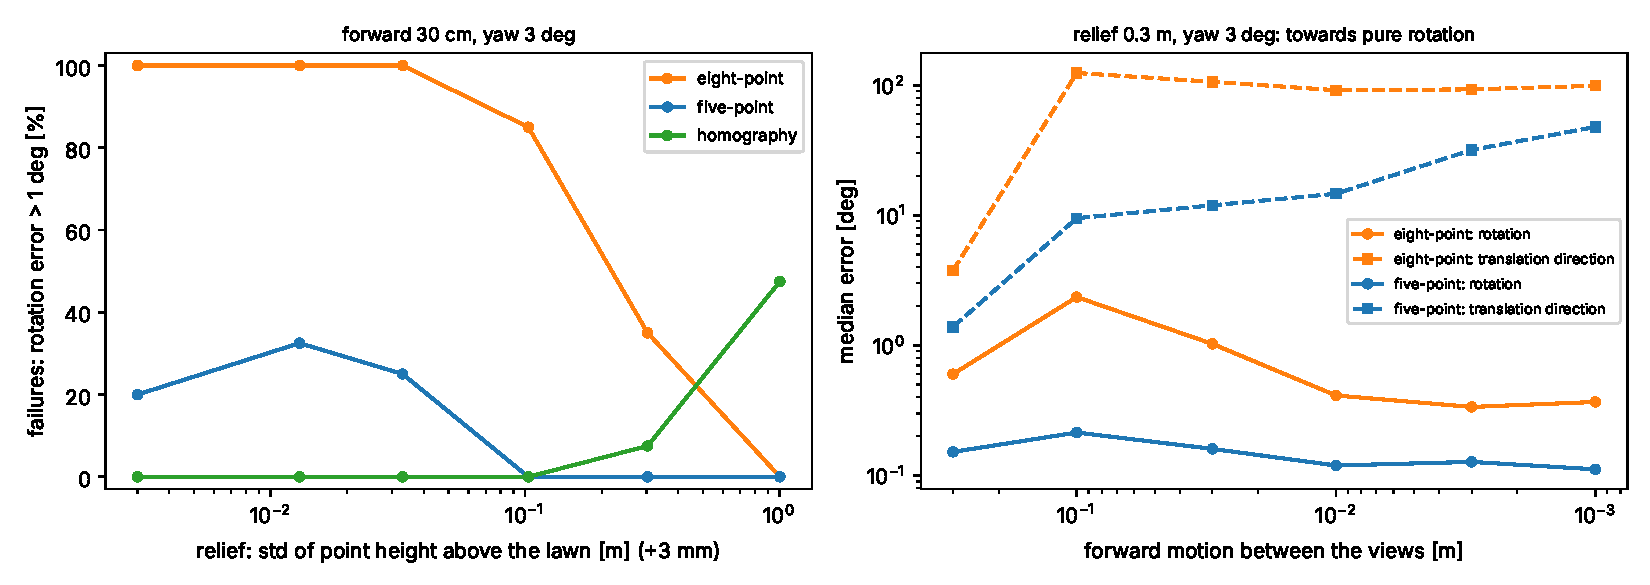
\includegraphics[width=\linewidth]{figures/ch06_degeneracy.pdf}
\caption{Relative pose from a mower camera 0.8\,m above the ground,
0.5\,px noise. Left: percentage of 40 trials with a rotation error above
$1^\circ$, as the scene goes from a perfect lawn to 1\,m of relief.
Eight-point fails on anything flat; five-point fails one time in four or
five on a lawn (the twin solution); the homography, disambiguated by the
known ground normal, never fails on a lawn but breaks once the scene has
real relief. Right: median errors as the forward motion shrinks towards
a pure rotation.}
\label{fig:degeneracy}
\end{figure}

\subsection{Turning on the spot}

\begin{proposition}{Pure rotation}{purerot}
If $\vect{t}=\vect0$, then $E=0$ and every correspondence satisfies
$\tilde{\vect{x}}_2\sim R\tilde{\vect{x}}_1$, whatever the depth of the
point. The rotation is determined; the translation direction and the
structure are not.
\end{proposition}

\begin{proof}
$E=\hatop{\vect0}R=0$, so \eqref{eq:epipolar} holds for any pair of
points and constrains nothing. $\vect{q}_2=R\vect{q}_1$ gives the
homography $R$ in normalised coordinates (Exercise~\ref{ex:3rot}); it
determines $R$, and contains no depth.
\end{proof}

Near this configuration, the translation direction becomes very poorly
determined while the rotation remains good (\cref{fig:degeneracy},
right: the five-point rotation error stays near $0.2^\circ$ while the
translation direction error grows from $1^\circ$ to $45^\circ$). The
right response is to recognise the situation --- the homography $R$
explains all matches --- and to update only the rotation, without
triangulating anything.

\begin{mower}
Two-view geometry on the PG98~HK:
\begin{itemize}[nosep]
\item \emph{Initialise on the ground plane.} On a lawn, the homography
  model with the known ground normal is the most reliable way to get the
  first relative pose and the first map; switch to the essential matrix
  as soon as the scene has relief (a hedge, a tree, a building).
\item \emph{Expect a blind spot ahead.} Forward motion leaves the centre
  of the image without parallax; points there are tracked but only
  triangulated once the mower turns or once they drift towards the image
  border.
\item \emph{Do not triangulate during turns on the spot}; use them to
  update the orientation only. The gyroscope of Chapter~12 does that job
  better anyway.
\item \emph{Scale is not in the images.} The translation of
  \cref{prop:decompose} has unit norm; the wheel odometry, the IMU or a
  stereo rig must supply the metres.
\end{itemize}
\end{mower}

\begin{practice}[\code{vslam/twoview.py}, \code{examples/ch06\_twoview.py},
  \code{notebooks/ch06\_twoview.ipynb}]
\begin{center}
\begin{tabular}{@{}ll@{}}
\toprule
Code & Formula\\
\midrule
\code{essential\_from\_pose}, \code{fundamental\_from\_essential} &
  \cref{prop:epipolar}\\
\code{eight\_point}, \code{project\_to\_essential} & eight-point
  algorithm\\
\code{demazure} & \cref{prop:demazure}\\
\code{sampson} & \cref{prop:sampson}\\
\code{decompose\_essential}, \code{recover\_pose} &
  \cref{prop:decompose}\\
\code{triangulate}, \code{parallax\_angle}, \code{in\_front} &
  \cref{prop:parallax}\\
\code{essential\_ransac}, \code{five\_point\_ransac} & RANSAC with 8 / 5
  points\\
\code{homography\_from\_plane}, \code{decompose\_homography} &
  \cref{prop:planar}\\
\bottomrule
\end{tabular}
\end{center}
The tests check the epipolar constraint, the singular values and cubic
constraints of $E$, the epipole of $F$, exact recovery by the eight-point
algorithm, that the four decompositions contain the truth and that
cheirality selects it, the Sampson distance against the exact distance to
the epipolar line, eight-point RANSAC with 30\,\% outliers, the rank
deficiency of a planar scene, the plane-induced homography and its
decomposition, and the parallax angle. The notebook draws epipolar
lines, prints the four candidates with their cheirality, compares the
three estimators on lawns and gardens, exhibits the twin solutions, and
implements the homography-or-essential decision.
\end{practice}

\section*{Further reading and C++ pointers}
\addcontentsline{toc}{section}{Further reading and C++ pointers}

Hartley and Zisserman, chapters~9--12, the reference for everything here.
H.~C.~Longuet-Higgins, ``A computer algorithm for reconstructing a scene
from two projections'', \emph{Nature}, 1981 (the essential matrix), and
``The reconstruction of a plane surface from two perspective
projections'', \emph{Proc.\ Royal Society B}, 1986; D.~Nist\'er, ``An
efficient solution to the five-point relative pose problem'', TPAMI 2004;
O.~Faugeras and F.~Lustman, 1988, and E.~Malis and M.~Vargas, 2007, for
homography decomposition; R.~Mur-Artal et al.\ (ORB-SLAM, 2015) for model
selection at initialisation. In C++: OpenCV's \code{findEssentialMat},
\code{recoverPose}, \code{triangulatePoints}, \code{findHomography} and
\code{decomposeHomographyMat}; OpenGV collects many relative-pose solvers.

\FloatBarrier
\section*{Exercises}
\addcontentsline{toc}{section}{Exercises}

\begin{enumerate}[label=\textbf{6.\arabic*},ref=6.\arabic*]
\item\label{ex:6epi} Show that $\vect{e}_2\T E=\vect0$ and $E\vect{e}_1=
  \vect0$ with $\vect{e}_2\sim\vect{t}$ and $\vect{e}_1\sim-R\T\vect{t}$,
  and that these are the images of the other camera's centre.
\item\label{ex:6twist} Show that the two rotations of
  \cref{prop:decompose} differ by a half-turn about the baseline:
  $(UW\T V\T)(UWV\T)\T$ is the rotation by $\pi$ about $\vect{u}_3$.
\item\label{ex:6fdof} Show that $F$ has rank 2 and seven degrees of
  freedom, and explain why a fundamental matrix need not have two equal
  singular values.
\item\label{ex:6forward} A mower drives 30\,cm straight ahead. Using
  \cref{prop:parallax}, estimate the parallax and the relative depth
  error ($f=500$\,px, $\sigma=0.5$\,px) of a tree 6\,m away, $10^\circ$
  off the direction of motion; then of the same tree $45^\circ$ off.
\end{enumerate}

\subsection*{Solutions}

\textbf{6.1.} $\vect{t}\T\hatop{\vect{t}}=-(\hatop{\vect{t}}\vect{t})\T
=\vect0\T$, so $\vect{t}\T E=\vect0$. And
$E(-R\T\vect{t})=-\hatop{\vect{t}}\vect{t}=\vect0$. The centre of
camera~1 has coordinates $\vect{q}_1=\vect0$, hence $\vect{q}_2=
\vect{t}$ in camera~2, whose image is $\tilde{\vect{x}}\sim\vect{t}$.
The centre of camera~2 has $\vect{q}_2=\vect0$, i.e.\ $\vect{q}_1=
-R\T\vect{t}$. Every epipolar line $\vect{l}_2=E\tilde{\vect{x}}_1$
satisfies $\vect{e}_2\T\vect{l}_2=0$: it passes through the epipole.

\textbf{6.2.} $(UW\T V\T)(VW\T U\T)=U(W\T)^2U\T$ and
$(W\T)^2=\diag(-1,-1,1)$, the rotation by $\pi$ about $\vect{e}_3$.
Conjugating by $U$ gives the rotation by $\pi$ about $U\vect{e}_3=
\vect{u}_3$, the direction of $\vect{t}$.

\textbf{6.3.} $F=K_2^{-\mathsf T}EK_1^{-1}$ with $K_i$ invertible has
the rank of $E$, i.e.\ 2. As a homogeneous matrix it has 8 degrees of
freedom, minus one for $\det F=0$: 7. Multiplication by $K_2^{-\mathsf
T}$ and $K_1^{-1}$ does not preserve singular values (these matrices are
not orthogonal), so the equal-singular-value property of $E$ is lost:
it is a property of calibrated cameras.

\textbf{6.4.} At $10^\circ$: $\theta\approx(0.3/6)\sin10^\circ=8.7
\times10^{-3}$\,rad $=0.50^\circ$. The depth error is of the order of
\cref{prop:parallax}(i), $\sqrt2\times0.5/(500\times8.7\times10^{-3})
\approx16\,\%$, i.e.\ about a metre. At $45^\circ$: $\theta\approx
0.035$\,rad $=2.0^\circ$ and the error is about $4\,\%$, 25\,cm. The same
tree is four times better triangulated when it is to the side.
